
%%%%%%%%%%%%%%%%%%%%%%%%%%%%%%%%%%%%%%%%%%%%%%%%%%%%%%%%%%%%%%%%%%%%%%%%%%%%%%
%  ************************** AVISO IMPORTANTE **************************    %
%                                                                            %
% Éste es un documento de ayuda para los autores que deseen enviar           %
% trabajos para su consideración en el Boletín de la Asociación Argentina    %
% de Astronomía.                                                             %
%                                                                            %
% Los comentarios en este archivo contienen instrucciones sobre el formato   %
% obligatorio del mismo, que complementan los instructivos web y PDF.        %
% Por favor léalos.                                                          %
%                                                                            %
%  -No borre los comentarios en este archivo.                                %
%  -No puede usarse \newcommand o definiciones personalizadas.               %
%  -SiGMa no acepta artículos con errores de compilación. Antes de enviarlo  %
%   asegúrese que los cuatro pasos de compilación (pdflatex/bibtex/pdflatex/ %
%   pdflatex) no arrojan errores en su terminal. Esta es la causa más        %
%   frecuente de errores de envío. Los mensajes de "warning" en cambio son   %
%   en principio ignorados por SiGMa.                                        %
%                                                                            %
%%%%%%%%%%%%%%%%%%%%%%%%%%%%%%%%%%%%%%%%%%%%%%%%%%%%%%%%%%%%%%%%%%%%%%%%%%%%%%

%%%%%%%%%%%%%%%%%%%%%%%%%%%%%%%%%%%%%%%%%%%%%%%%%%%%%%%%%%%%%%%%%%%%%%%%%%%%%%
%  ************************** IMPORTANT NOTE ******************************  %
%                                                                            %
%  This is a help file for authors who are preparing manuscripts to be       %
%  considered for publication in the Boletín de la Asociación Argentina      %
%  de Astronomía.                                                            %
%                                                                            %
%  The comments in this file give instructions about the manuscripts'        %
%  mandatory format, complementing the instructions distributed in the BAAA  %
%  web and in PDF. Please read them carefully                                %
%                                                                            %
%  -Do not delete the comments in this file.                                 %
%  -Using \newcommand or custom definitions is not allowed.                  %
%  -SiGMa does not accept articles with compilation errors. Before submission%
%   make sure the four compilation steps (pdflatex/bibtex/pdflatex/pdflatex) %
%   do not produce errors in your terminal. This is the most frequent cause  %
%   of submission failure. "Warning" messsages are in principle bypassed     %
%   by SiGMa.                                                                %
%                                                                            % 
%%%%%%%%%%%%%%%%%%%%%%%%%%%%%%%%%%%%%%%%%%%%%%%%%%%%%%%%%%%%%%%%%%%%%%%%%%%%%%

\documentclass[baaa]{baaa}
\usepackage[spanish]{babel}
\usepackage{siunitx} % Para manejo de unidades e incertidumbres
\usepackage{booktabs} % Para líneas de tabla de calidad profesional
\usepackage{multirow} % Para celdas combinadas

%%%%%%%%%%%%%%%%%%%%%%%%%%%%%%%%%%%%%%%%%%%%%%%%%%%%%%%%%%%%%%%%%%%%%%%%%%%%%%
%  ******************** Paquetes Latex / Latex Packages *******************  %
%                                                                            %
%  -Por favor NO MODIFIQUE estos comandos.                                   %
%  -Si su editor de texto no codifica en UTF8, modifique el paquete          %
%  'inputenc'.                                                               %
%                                                                            %
%  -Please DO NOT CHANGE these commands.                                     %
%  -If your text editor does not encodes in UTF8, please change the          %
%  'inputec' package                                                         %
%%%%%%%%%%%%%%%%%%%%%%%%%%%%%%%%%%%%%%%%%%%%%%%%%%%%%%%%%%%%%%%%%%%%%%%%%%%%%%
 
\usepackage[pdftex]{hyperref}
\usepackage{subfigure}
\usepackage{natbib}
\usepackage{helvet,soul}
\usepackage[font=small]{caption}
\usepackage[spanish]{babel}
\usepackage{booktabs} % Para líneas más limpias
\usepackage{siunitx}  % Para alinear números y unidades
\usepackage{caption} % Paquete necesario para personalizar
\captionsetup[figure]{name=FIG, labelsep=period} % Cambia "Figura" por "FIG"
\captionsetup[table]{name=TABLA, labelsep=period} % Cambia "Table" por "TABLA"
\usepackage{appendix} % Para manejo de anexos
\usepackage{afterpage} % Para control de paginación
\usepackage{siunitx}


%%%%%%%%%%%%%%%%%%%%%%%%%%%%%%%%%%%%%%%%%%%%%%%%%%%%%%%%%%%%%%%%%%%%%%%%%%%%%%
%  *************************** Idioma / Language **************************  %
%                                                                            %
%  -Ver en la sección 3 "Idioma" para mas información                        %
%  -Seleccione el idioma de su contribución (opción numérica).               %
%  -Todas las partes del documento (titulo, texto, figuras, tablas, etc.)    %
%   DEBEN estar en el mismo idioma.                                          %
%                                                                            %
%  -Select the language of your contribution (numeric option)                %
%  -All parts of the document (title, text, figures, tables, etc.) MUST  be  %
%   in the same language.                                                    %
%                                                                            %
%  0: Castellano / Spanish                                                   %
%  1: Inglés / English                                                       %
%%%%%%%%%%%%%%%%%%%%%%%%%%%%%%%%%%%%%%%%%%%%%%%%%%%%%%%%%%%%%%%%%%%%%%%%%%%%%%

\contriblanguage{1}

%%%%%%%%%%%%%%%%%%%%%%%%%%%%%%%%%%%%%%%%%%%%%%%%%%%%%%%%%%%%%%%%%%%%%%%%%%%%%%
%  *************** Tipo de contribución / Contribution type ***************  %
%                                                                            %
%  -Seleccione el tipo de contribución solicitada (opción numérica).         %
%                                                                            %
%  -Select the requested contribution type (numeric option)                  %
%                                                                            %
%  1: Artículo de investigación / Research article                           %
%  2: Artículo de revisión invitado / Invited review                         %
%  3: Mesa redonda / Round table                                             %
%  4: Artículo invitado  Premio Varsavsky / Invited report Varsavsky Prize   %
%  5: Artículo invitado Premio Sahade / Invited report Sahade Prize          %
%  6: Artículo invitado Premio Sérsic / Invited report Sérsic Prize          %
%%%%%%%%%%%%%%%%%%%%%%%%%%%%%%%%%%%%%%%%%%%%%%%%%%%%%%%%%%%%%%%%%%%%%%%%%%%%%%

\contribtype{1}

%%%%%%%%%%%%%%%%%%%%%%%%%%%%%%%%%%%%%%%%%%%%%%%%%%%%%%%%%%%%%%%%%%%%%%%%%%%%%%
%  ********************* Área temática / Subject area *********************  %
%                                                                            %
%  -Seleccione el área temática de su contribución (opción numérica).        %
%                                                                            %
%  -Select the subject area of your contribution (numeric option)            %
%                                                                            %
%  1 : SH    - Sol y Heliosfera / Sun and Heliosphere                        %
%  2 : SSE   - Sistema Solar y Extrasolares  / Solar and Extrasolar Systems  %
%  3 : AE    - Astrofísica Estelar / Stellar Astrophysics                    %
%  4 : SE    - Sistemas Estelares / Stellar Systems                          %
%  5 : MI    - Medio Interestelar / Interstellar Medium                      %
%  6 : EG    - Estructura Galáctica / Galactic Structure                     %
%  7 : AEC   - Astrofísica Extragaláctica y Cosmología /                      %
%              Extragalactic Astrophysics and Cosmology                      %
%  8 : OCPAE - Objetos Compactos y Procesos de Altas Energías /              %
%              Compact Objetcs and High-Energy Processes                     %
%  9 : ICSA  - Instrumentación y Caracterización de Sitios Astronómicos
%              Instrumentation and Astronomical Site Characterization        %
% 10 : AGE   - Astrometría y Geodesia Espacial
% 11 : ASOC  - Astronomía y Sociedad                                             %
% 12 : O     - Otros
%
%%%%%%%%%%%%%%%%%%%%%%%%%%%%%%%%%%%%%%%%%%%%%%%%%%%%%%%%%%%%%%%%%%%%%%%%%%%%%%

\thematicarea{99}

%%%%%%%%%%%%%%%%%%%%%%%%%%%%%%%%%%%%%%%%%%%%%%%%%%%%%%%%%%%%%%%%%%%%%%%%%%%%%%
%  *************************** Título / Title *****************************  %
%                                                                            %
%  -DEBE estar en minúsculas (salvo la primer letra) y ser conciso.          %
%  -Para dividir un título largo en más líneas, utilizar el corte            %
%   de línea (\\).                                                           %
%                                                                            %
%  -It MUST NOT be capitalized (except for the first letter) and be concise. %
%  -In order to split a long title across two or more lines,                 %
%   please use linebreaks (\\).                                              %
%%%%%%%%%%%%%%%%%%%%%%%%%%%%%%%%%%%%%%%%%%%%%%%%%%%%%%%%%%%%%%%%%%%%%%%%%%%%%%
% Dates
% Only for editors
\received{\ldots}
\accepted{\ldots}




%%%%%%%%%%%%%%%%%%%%%%%%%%%%%%%%%%%%%%%%%%%%%%%%%%%%%%%%%%%%%%%%%%%%%%%%%%%%%%



\title{Una apresurada introducción a los resultados, teóricos y empíricos, de la estadística, la probabilidad, la programación y, tal vez, de la (pseudo)aleatoriedad}

%%%%%%%%%%%%%%%%%%%%%%%%%%%%%%%%%%%%%%%%%%%%%%%%%%%%%%%%%%%%%%%%%%%%%%%%%%%%%%
%  ******************* Título encabezado / Running title ******************  %
%                                                                            %
%  -Seleccione un título corto para el encabezado de las páginas pares.      %
%                                                                            %
%  -Select a short title to appear in the header of even pages.              %
%%%%%%%%%%%%%%%%%%%%%%%%%%%%%%%%%%%%%%%%%%%%%%%%%%%%%%%%%%%%%%%%%%%%%%%%%%%%%%

\titlerunning{Introducción a la probabilidad, la estadística, y los numeros aleatorios}

%%%%%%%%%%%%%%%%%%%%%%%%%%%%%%%%%%%%%%%%%%%%%%%%%%%%%%%%%%%%%%%%%%%%%%%%%%%%%%
%  ******************* Lista de autores / Authors list ********************  %
%                                                                            %
%  -Ver en la sección 3 "Autores" para mas información                       % 
%  -Los autores DEBEN estar separados por comas, excepto el último que       %
%   se separar con \&.                                                       %
%  -El formato de DEBE ser: S.W. Hawking (iniciales luego apellidos, sin     %
%   comas ni espacios entre las iniciales).                                  %
%                                                                            %
%  -Authors MUST be separated by commas, except the last one that is         %
%   separated using \&.                                                      %
%  -The format MUST be: S.W. Hawking (initials followed by family name,      %
%   avoid commas and blanks between initials).                               %
%%%%%%%%%%%%%%%%%%%%%%%%%%%%%%%%%%%%%%%%%%%%%%%%%%%%%%%%%%%%%%%%%%%%%%%%%%%%%%

\author{
V.R. Sandez\inst{1,2},
}

\authorrunning{SANDEZ}

%%%%%%%%%%%%%%%%%%%%%%%%%%%%%%%%%%%%%%%%%%%%%%%%%%%%%%%%%%%%%%%%%%%%%%%%%%%%%%
%  **************** E-mail de contacto / Contact e-mail *******************  %
%                                                                            %
%  -Por favor provea UNA ÚNICA dirección de e-mail de contacto.              %
%                                                                            %
%  -Please provide A SINGLE contact e-mail address.                          %
%%%%%%%%%%%%%%%%%%%%%%%%%%%%%%%%%%%%%%%%%%%%%%%%%%%%%%%%%%%%%%%%%%%%%%%%%%%%%%

\contact{ruben.sandez@unc.edu.ar}

%%%%%%%%%%%%%%%%%%%%%%%%%%%%%%%%%%%%%%%%%%%%%%%%%%%%%%%%%%%%%%%%%%%%%%%%%%%%%%
%  ********************* Afiliaciones / Affiliations **********************  %
%                                                                            %
%  -La lista de afiliaciones debe seguir el formato especificado en la       %
%   sección 3.4 "Afiliaciones".                                              %
%                                                                            %
%  -The list of affiliations must comply with the format specified in        %          
%   section 3.4 "Afiliaciones".                                              %
%%%%%%%%%%%%%%%%%%%%%%%%%%%%%%%%%%%%%%%%%%%%%%%%%%%%%%%%%%%%%%%%%%%%%%%%%%%%%%

\institute{
Observatorio Astron\'omico de C\'ordoba, UNC, Argentina
\and
Facultad de Matemáticas, Astronomía, Física y Computación, UNC, Argentina
}

%%%%%%%%%%%%%%%%%%%%%%%%%%%%%%%%%%%%%%%%%%%%%%%%%%%%%%%%%%%%%%%%%%%%%%%%%%%%%%
%  *************************** Resumen / Summary **************************  %
%                                                                            %
%  -Ver en la sección 3 "Resumen" para mas información                       %
%  -Debe estar escrito en castellano y en inglés.                            %
%  -Debe consistir de un solo párrafo con un máximo de 1500 (mil quinientos) %
%   caracteres, incluyendo espacios.                                         %
%                                                                            %
%  -Must be written in Spanish and in English.                               %
%  -Must consist of a single paragraph with a maximum  of 1500 (one thousand %
%   five hundred) characters, including spaces.                              %
%%%%%%%%%%%%%%%%%%%%%%%%%%%%%%%%%%%%%%%%%%%%%%%%%%%%%%%%%%%%%%%%%%%%%%%%%%%%%%

 \resumen{En este trabajo }

\abstract{En este breve informe se mostraran los resultados obtenidos al hacer un estudio numérico/computacional a cerca de las nociones y propiedades básicas relacionadas a la probabilidad, la estadística y los números aleatorios. Compararemos los resultados arrojados por los algorítmos con los resultados teoricos para determinar cuales son los mejores algoritmos para cada tarea. Posteriormente se aplicarán estos algoritmos en problemas específicos para darle un uso interesante.}

%%%%%%%%%%%%%%%%%%%%%%%%%%%%%%%%%%%%%%%%%%%%%%%%%%%%%%%%%%%%%%%%%%%%%%%%%%%%%%
%                                                                            %
%  Seleccione las palabras clave que describen su contribución. Las mismas   %
%  son obligatorias, y deben tomarse de la lista de la American Astronomical %
%  Society (AAS), que se encuentra en la página web indicada abajo.          %
%                                                                            %
%  Select the keywords that describe your contribution. They are mandatory,  %
%  and must be taken from the list of the American Astronomical Society      %
%  (AAS), which is available at the webpage quoted below.                    %
%                                                                            %
%  https://journals.aas.org/keywords-2013/                                   %
%                                                                            %
%%%%%%%%%%%%%%%%%%%%%%%%%%%%%%%%%%%%%%%%%%%%%%%%%%%%%%%%%%%%%%%%%%%%%%%%%%%%%%

\keywords{ Astrostatistics - Probability - Random Numers - Fibonacci Generator - Random Walks -Monty Hall }

\begin{document}

\maketitle

\section{Introducción}\label{S_intro}

La generación de números aleatorios y el estudio de métodos probabilísticos constituyen pilares fundamentales en la astroestadística moderna. En un campo donde los fenómenos observados son intrínsecamente estocásticos y donde los experimentos controlados son imposibles de realizar, la capacidad de simular procesos astronómicos mediante números aleatorios se convierte en una herramienta indispensable.

El dominio de estas técnicas no es meramente académico; constituye una habilidad práctica esencial para cualquier astrofísico moderno. La capacidad de generar, validar y utilizar secuencias aleatorias de alta calidad diferencia entre resultados científicos robustos y conclusiones potencialmente erróneas. Este estudio sienta las bases para métodos computacionales más avanzados que son estándar en la investigación astronómica contemporánea.

\subsection{ El lenguaje de la Astronomía Contemporánea}
La revolución computacional en astronomía ha encontrado en Python su plataforma por defecto para desarrollarse. La elección de Python como lenguaje principal para estos ejercicios no es arbitraria sino que responde a razones pragmáticas que lo han convertido en el estándar de facto en la investigación astronómica mundial. Mucha gente cuestiona al día de hoy esta decisión colectiva, proponiendo alternativas que poco satisfacen las necesidades de los usuarios investigadores.

A lo largo de los años la comunidad de usuarios de Python Ha generado un ecosistema para el desarrollo de la ciencia sin precedentes, y es por eso que su uso se ha extendido tanto. La generación de \textit{librerias} de uso público han facilitado el trabajo de todos.

Entre otras muchas cosas, podemos decir, que Python ha democratizado el acceso a herramientas computacionales avanzadas que antes estaban reservadas para especialistas en computación. Hoy, cualquier astrónomo puede implementar algoritmos complejos, analizar terabytes de datos y realizar simulaciones sofisticadas gracias a este ecosistema.

Esta combinación de poder computacional, accesibilidad y robustez estadística hace de Python la elección ideal para formar a la próxima generación de astrofísicos computacionales.

\section{Metodología}

Para el estudio de estos fenómenos se generó un \texttt{Jupyter Notebook} donde se detallan los algoritmos y programas implementados para cada tarea. El mismo se encuentra en el repositorio \textbf{https://github.com/rubsanmon22/2025-unc-famaf-astro-astrometria1} en la carpeta \texttt{tp1}. A su vez, se generó un archivo \texttt{rubfx.py}, parte de la misma carpeta, que fue recopilando las funciones necesarias para poder ejecutar los algoritmos en cada etapa.

\subsection{Generador Lineal de Congruencias}

En primera instancia se introduce la idea de la generación de números pseudoaleatorios mediante el método de congruencia lineal, uno de los algoritmos más fundamentales en la historia de la simulación computacional. Este algoritmo no solo tiene valor histórico, sino que sienta las bases para entender cómo las computadoras generan "aleatoriedad" controlada.

La importancia de este algoritmo radica en la necesidad de simular distribuciones, generar catálogos sintéticos, realizar integraciones Monte Carlo, crear muestras de control para experimentos, etc.

Siguiendo la bibliografía de la materia, particularmente The Nature of Mathematical Modelling \citep{gershenfeld1998nature}, entendemos al Generador Lineal Congruencial de números aleatorios (y sus variantes) como una técnica fundamental para la producción de números pseudoaleatorios en computación.

El método se define mediante la fórmula de recurrencia:

\begin{equation}
    x_{n+1} = (a \cdot x_n + c) \mod M
\end{equation}

Esta ecuación lineal, aparentemente simple, genera secuencias de números que exhiben pseudoaleatoriedad. Sin embargo, es crucial reconocer que detrás de esta apariencia aleatoria se esconden patrones determinísticos, cuya detección requiere un análisis estadístico riguroso. Las variables de este modelo son: \textbf{$x_n$}: Estado actual, \textbf{$a$}: Multiplicador, \textbf{$b$}: Incremento, \textbf{$M$}: Módulo.

La elección de estos parámetros es crítica para la calidad del generador. Dada una semilla inicial, se deben seleccionar parámetros que minimicen las correlaciones seriales y maximicen el período de la secuencia generada.

La finalidad es implementar este algoritmo de manera que, al iterar la operación, se obtenga una secuencia de números en el rango [0,1] con correlaciones mínimas a escalas grandes, adecuada para aplicaciones astroestadísticas.

Para poder dar cuenta de la \textit{uniformidad} de este generador necesitamos un histograma que de cuenta de la distribución de números y ver que la misma no esté sesgada de alguna manera.

\subsection{Comparación numérica vs. teórica}

Otra forma de analizar la distribución, particularmente aquella donde vemos números entre 0 y 1, es analizando los \textit{momentos} de la distribución. Una medida estadística que nos ayuda a comprar el comportamiento real con el comportamiento "teorico" esperado \citep{gershenfeld1999nature}.

Para una distribución teorica continua, uniforme donde $f(x)=1$ en [0,1] tenemos por definición:

Momento de orden $k$ teórico

\begin{equation}
\centering
\mu_{k}=E[X^k] = \int_0^1 x^k \cdot 1  dx = \frac{1}{k+1}
\end{equation}

Al contar con una distribución discreta, la integral se convierte en una sumatoria, definida como momento empírico:

\begin{equation}
\centering
\hat{\mu}_k = \frac{1}{n} \sum_{i=1}^n x_i^k
\end{equation}

El objetivo de todo esto es ver que, en el infinito, a mayor numero de n vale $ \mu_{k} = \hat{\mu}_k$. Entonces podemos decir que:

\begin{equation}
\centering
\lim_{n \to \infty} \hat{\mu}_k = \mu_{k}
\end{equation}

\begin{equation}
\centering
\lim_{n \to \infty} \frac{1}{n} \sum_{i=1}^n x_i^k = \int_0^1 x^k \cdot 1  dx 
\end{equation}

Numericamente podriamos intentar corroborar esta afirmación. Veamos entonces que se cumple: 

\begin{equation}
\centering
\lim_{n \to \infty} \frac{1}{n} \sum_{i=1}^n x_i^k = \frac{1}{k+1}
\end{equation}

En general asociamos a cada momento una noción de significado, como media, desviación estándar, etc. En este trabajo solo lo utilizaremos como medidor de calidad para comparar el valor teórico esperado con el valor calculado por la máquina.

\subsection{\textit{Random Walk}}

Una forma interesante de implementar este algoritmo es estudiar el \textit{random walk}, útil para modelar ciertos fenómenos físicos, como el movimiento browniano, la difusión de calor y demás fenómenos \textit{estocásticos} complejos.

Esto es tan simple como ubicar en la coordenadas $x$ e $y$ un generador de numero aleatorio con semilla que vaya recorriendo valores entre $-a$ y $a$, con lo cual, usando la función generadora de congruencias lineales, y reescalándola, obtendremos lo que buscamos. Este tiene un comportamiento teórico esperado, cada paso en la caminata es un $\Delta \vec{r_i}=(\Delta x_i,\Delta y_i)$. Luego de dar N pasos el valor el valor será $\vec R_N=\sum_{i=1}^{N} \Delta \vec{r_i}=(X_N, Y_N)$. Entonces la distancia al orgien es $R_N = \|\vec {R_N}\|=\sqrt{X_N²+Y_N²}$. 

Este valor lo queremos comparar con su evolución en pasos y posteriormente con su evolicion en función de $\sqrt{n}$. Veremos finalmente que $R_N \propto \sqrt{N}$.

\subsection{Fibonacci, otro generador}

De momento vimos aplicaciones básicas para generar números pseudoaleatorios y su uso en el cálculo de momentos y caminatas aleatorias.

Ahora bien, este no es el único algoritmo que tenemos para generar números pseudoaleatorios. Un nuevo gran ejemplo de esto es el \textit{Generador de Fibonacci con Retardo}.

\begin{equation}
\centering
X_n = (X_{n-j} + X_{n-k}) \bmod m
\end{equation}

Donde \( X_n \) es el \( n \)-ésimo término de la secuencia pseudoaleatoria, \( j \) y \( k \) (con \( j < k \)) son los \textit{retardos} que determinan cuán atrás en la secuencia se toman los valores para combinar, \( \star \) representa una operación que actúa sobre dichos valores, y \( m \) es el módulo.

\subsection{Coeficiente de Pearson}

Una forma de cuantificar el grado de relación que tienen dos variables cuantitativas es a través del \textit{Coeficiente de Correlación de Pearson.} 

El coeficiente de correlación de Pearson se define mediante la siguiente expresión matemática:

\begin{equation}
r = \frac{\sum\limits_{i=1}^{n} (x_i - \bar{x})(y_i - \bar{y})}{\sqrt{\sum\limits_{i=1}^{n} (x_i - \bar{x})^2 \sum\limits_{i=1}^{n} (y_i - \bar{y})^2}}
\end{equation}

donde $n$ representa el número de observaciones, $x_i$ e $y_i$ son los valores individuales de las variables, y $\bar{x}$ e $\bar{y}$ corresponden a las medias muestrales de $x$ e $y$ respectivamente.

¿Qué significado del valor? Si este es muy cercano a 0: Indica que no existe una relación lineal apreciable entre las variables.

Cuando se encuentre en el rango: -1 (correlación negativa perfecta) a +1 (correlación positiva perfecta). Esto es decir que hay una relación inversamente proporcional, o proporcional, respectivamente, entre las variables. 

Si nosotros quisiéramos calcular cuán correlacionados están dos generadores, deberíamos usar esta relación. 

\subsection{Aplicaciones de los algoritmos}

Cualquier generador de números pseudoaleatorios, implementado mediante el método de congruencia lineal o el generador fibonacci, constituye la herramienta fundamental para la simulación de procesos estocásticos en diversos problemas. Su función principal es generar secuencias de números entre 0 y 1, los cuales posteriormente son transformados para emular el comportamiento aleatorio de cada sistema bajo estudio.

\subsubsection{Monty Hall}
El generador se utiliza para simular múltiples realizaciones del juego. En cada iteración:
\begin{itemize}


\item Se genera un número aleatorio para determinar la puerta que oculta el automóvil (1, 2, 3).

\item Se genera otro valor para simular la elección inicial del participante.

\item Se implementa la regla del presentador (abrir una puerta con cabra).

\item Se evalúan ambas estrategias: «mantener la elección inicial» y «cambiar de puerta».

\end{itemize}
La probabilidad de éxito de cada estrategia se estima mediante la frecuencia relativa de victorias sobre un número grande de simulaciones.

\subsubsection{Tipos de Galaxias}
Mediante el muestreo por transformación inversa a partir de la distribución discreta dada, el generador permite crear catálogos sintéticos de galaxias. Para cada galaxia:
\begin{equation*}
\text{Tipo} = 
\begin{cases}
\text{Elíptica}    & \text{si } u \in [0, 0.4) \\
\text{Espiral}     & \text{si } u \in [0.4, 0.7) \\
\text{Enana}       & \text{si } u \in [0.7, 0.9) \\
\text{Irregular}   & \text{si } u \in [0.9, 1.0)
\end{cases}
\end{equation*}
donde $u$ es un número aleatorio generado a partir de la secuencia pseudoaleatoria.

\subsubsection{Suma de Dos Dados}
El generador se emplea para simular el lanzamiento de dos dados equilibrados. Para cada dado:
\begin{equation*}
\text{Resultado} = \lfloor 6 \cdot u \rfloor + 1
\end{equation*}
donde $u$ es un número entre 0 y 1. La variable aleatoria se calcula como la adición de los resultados de ambos dados. La distribución empírica resultante se compara con la distribución teórica para validar el método de simulación.

En todos los casos, el generador de congruencia lineal provee la secuencia base $\{u_n\}$, la cual es adaptada mediante transformaciones o reescalamientos para emular las variables aleatorias buscada.



\section{Resultados - Funciones}

\subsection{Comportamiento del Generador Lineal de Congruencias}

En primera instancia definimos la función \texttt{rfx.gclz()}, dentro de las funciones \texttt{rubfx.py}, como un \textit{Generador Lineal de Congruencias}, que genere numeros aleatorios entre $0$ y $m-1$, a los que le asociamos los siguientes parámetros:$x_0=10$, $a=57$, $c=1$, $m=256$, $n=256$. Estos valores nos arrojan una distribución que, a pequeña escala, cuando los graficamos, parecieran no presentar ningun patrón o correlación (ver Fig. \ref{gclz256}).

\begin{figure}[!h]
    \centering
    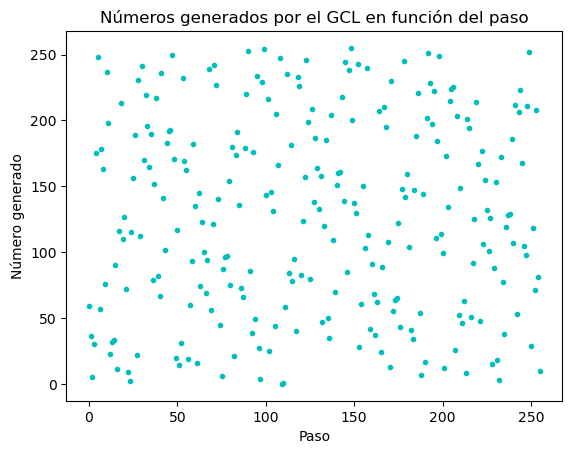
\includegraphics[width=0.9\linewidth]{imagenes/gclz256.png}
    \caption{Distribución de números generados para los valores $x_0=10$, $a=57$, $c=1$, $m=256$, $n=256$.}
    \label{gclz256}
\end{figure}

Al aumentar el número $n$ (ver Fig. \ref{gclz5000}) la cosa cambia, notamos un patrón claro y deja en claro que la elección de números es objetivamente mala.

\begin{figure}[!h]
    \centering
    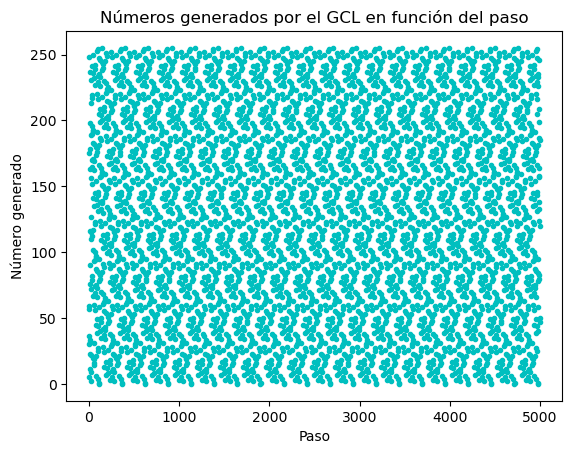
\includegraphics[width=0.9\linewidth]{imagenes/gclz5000.png}
    \caption{Distribución de números generados para los valores $x_0=10$, $a=57$, $c=1$, $m=256$, $n=5000$.}
    \label{gclz5000}
\end{figure}

Aumentando el número de datos vemos de manera obvia que el patrón tiende a repetirse, lo cual nos deja clarísimo que esta función es \textit{determinista}. Cambiando distintas variables, como la semilla, o el módulo vemos patrones más o menos notables.

Para ver cuanta uniformidad puede alcanzar a altos números de $n$, realizamos un histograma (ver Fig. \ref{histogclz5000})que deja en evidencia varias cuestiones.

\begin{figure}[!h]
    \centering
    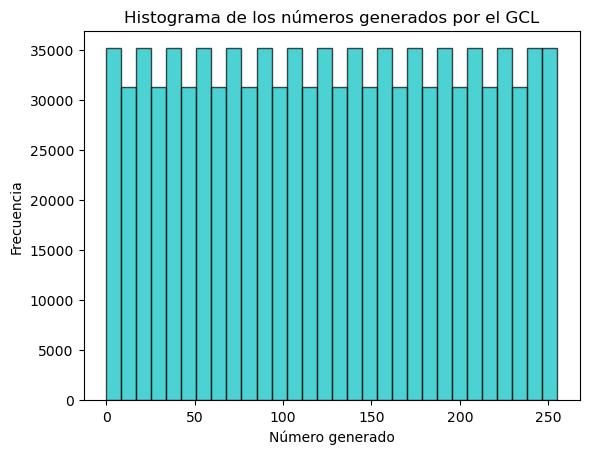
\includegraphics[width=0.9\linewidth]{imagenes/histogclz5000.png}
    \caption{Histograma para la distribución de números generados para los valores $x_0=10$, $a=57$, $c=1$, $m=256$, $n=5000$.}
    \label{histogclz5000}
\end{figure}

Se detectan pequeñas variaciones dentro de la normalidad, relacionadas a la \textit{ley de grandes números}. En definitiva, esta elección de números no es la adecuada para trabajar con pseudoaleatoriedad.

Todos estos defectos son generados por nuestra elección de constantes que definen el generador.

A lo largo de los años hemos podido encontrar mejores parámetros donde estos patrones son dificiles de detectar. No solo son mejores en cuanto a \textit{aleatoriedad}, sino tambien son mas eficientes en terminos computacionales.

Uno de los más famosos es el propuesto en el libro \textit{Numerical Recipes}\citep{teukolsky1992numerical}, donde se toman los siguientes valores: $a=1664525$, $c=1013904223$, $m=2^{32}$. Como la comparación a pequeña escala no tiene sentido buscamos directamente comparar con un valor dado para $n=5000$ y usando la misma semilla (ver Fig. \ref{gclzb5000}). 

\begin{figure}[!h]
    \centering
    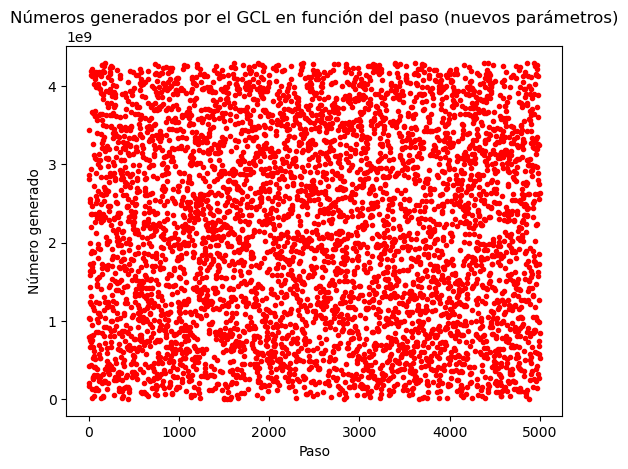
\includegraphics[width=0.9\linewidth]{imagenes/gclzb5000.png}
    \caption{Distribución de números generados para los valores $x_0=10$, $a=1664525$, $c=1013904223$, $m=2^{32}$, $n=5000$. }
    \label{gclzb5000}
\end{figure}


Con esta nueva distribución la aleatorieda pareciera estar practicamente asegurada, las correlaciones no son obvias y solo un analisis suficientemente bueno podria detectarlas. Los defectos de la anterior distribución dejan de ser tan notables (ver Fig. \ref{histogclzb5000}).

\begin{figure}[!h]
    \centering
    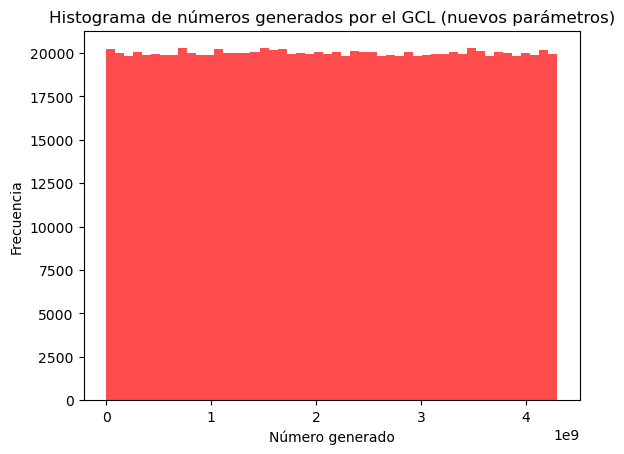
\includegraphics[width=0.9\linewidth]{imagenes/histogclzb5000.png}
    \caption{Histograma para la distribución de números generados para los valores $x_0=10$, $a=1664525$, $c=1013904223$, $m=2^{32}$, $n=5000$.}
    \label{histogclzb5000}
\end{figure}

A partir de ahora usaremos esta configuración para la función \texttt{rfx.gclz()}.

\subsection{Los momentos de la distribución generada}

Se generaron las funciones \texttt{rfx.momt()}, \texttt{rfx.mome()}, que calculan los momentos teóricos y empíricos de las distribuciones generadas por la función \texttt{rfx.gclz()}. Con los resultados de cada momento podemos comparar los resultados a distintos valores de $n$, también podemos calcular los errores relativos entre estos para interpretar mejor los resultados.  

\begin{table*}[h!]
\centering
\scriptsize
\caption{Comparación completa de momentos teóricos, empíricos y errores relativos}
\label{momentos}
\resizebox{\textwidth}{!}{%
\begin{tabular}{c S[table-format=1.6] *{12}{S[table-format=1.6]}}
\toprule
\multirow{2}{*}{$k$} & \multirow{2}{*}{Teórico} & \multicolumn{2}{c}{$n=10$} & \multicolumn{2}{c}{$n=100$} & \multicolumn{2}{c}{$n=1,000$} & \multicolumn{2}{c}{$n=10,000$} & \multicolumn{2}{c}{$n=100,000$} & \multicolumn{2}{c}{$n=1,000,000$} \\
\cmidrule(lr){3-4} \cmidrule(lr){5-6} \cmidrule(lr){7-8} \cmidrule(lr){9-10} \cmidrule(lr){11-12} \cmidrule(lr){13-14}
 & & {Emp.} & {Error} & {Emp.} & {Error} & {Emp.} & {Error} & {Emp.} & {Error} & {Emp.} & {Error} & {Emp.} & {Error} \\
\midrule
1 & 0.500000 & 0.348472 & 0.303055 & 0.441043 & 0.117914 & 0.485543 & 0.028915 & 0.497414 & 0.005172 & 0.498491 & 0.003017 & 0.499794 & 0.000413 \\
2 & 0.333333 & 0.199872 & 0.400384 & 0.291076 & 0.126771 & 0.323319 & 0.030043 & 0.331192 & 0.006423 & 0.331829 & 0.004513 & 0.333087 & 0.000739 \\
3 & 0.250000 & 0.132682 & 0.469270 & 0.223252 & 0.106990 & 0.244007 & 0.023972 & 0.248355 & 0.006581 & 0.248604 & 0.005585 & 0.249763 & 0.000947 \\
4 & 0.200000 & 0.092381 & 0.538095 & 0.184316 & 0.078420 & 0.196582 & 0.017088 & 0.198584 & 0.007080 & 0.198706 & 0.006471 & 0.199788 & 0.001062 \\
5 & 0.166667 & 0.065792 & 0.605251 & 0.158807 & 0.047156 & 0.164842 & 0.010946 & 0.165323 & 0.008059 & 0.165460 & 0.007239 & 0.166479 & 0.001129 \\
6 & 0.142857 & 0.047589 & 0.666876 & 0.140624 & 0.015629 & 0.142023 & 0.005839 & 0.141515 & 0.009392 & 0.141727 & 0.007913 & 0.142690 & 0.001173 \\
7 & 0.125000 & 0.034876 & 0.720990 & 0.126875 & 0.015001 & 0.124785 & 0.001721 & 0.123632 & 0.010944 & 0.123937 & 0.008504 & 0.124849 & 0.001208 \\
8 & 0.111111 & 0.025862 & 0.767238 & 0.116014 & 0.044129 & 0.111281 & 0.001531 & 0.109709 & 0.012618 & 0.110109 & 0.009018 & 0.110973 & 0.001239 \\
\bottomrule
\end{tabular}%
}
\end{table*}

Notamos claramente como a medida que la muestra aumenta, menor se hacen los errores (ver Tabla \ref{momentos}). De hecho, disminuyen de forma exponencial (ver Fig. \ref{errel}).

Se nota que hay un máximo de divergencia al rededor del valor $10³$, luego los errores son similares entre si, hacercandose cada vez mas entre si.

O sea, a grandes valores de n, el valor de los errores absolutos entre los momentos es siempre menor.

\begin{figure}[!h]
    \centering
    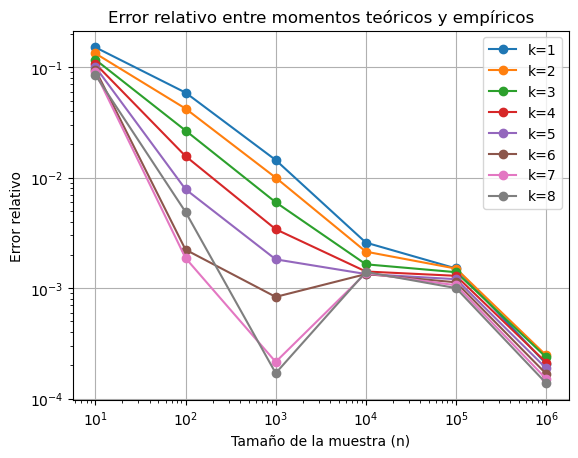
\includegraphics[width=0.9\linewidth]{imagenes/errel.png}
    \caption{Error relativo entre momentos teóricos y empíricos.}
    \label{errel}
\end{figure}

\subsection{Caminata aleatoria entre $-\sqrt{2}$ y $\sqrt{2}$}
Ahora buscamos implementar de manera directa el \texttt{rfx.glcr()} (La función que genera numeros entre 0 y 1 basada en \texttt{rfx.glcz()}.), particularmente para estudiar el \textit{random walk}, util para modelar ciertos fenomenos físicos como el movimiento browniano, la difusión de calor y demás fenomenos \textit{estocásticos} complejos.

Esto es tan simple como ubicar en la coordenadas $x$ e $y$ un generador de numero aleatorio con semilla que vaya recorriendo valores entre $-\sqrt{2}$ y $\sqrt{2}$, con lo cual, usando la función gclr, y reescalandola, obtendremos lo que buscamos.

Vemos que a simple vista no hay ninguna correlación clara (ver Fig. \ref{randomwalk}), aunque vemos que la caminata no se extiende tanto en el espacio como uno tal vez esperaría. Para cuantificar de alguna forma este comportamiento tratamos de determinar el valor $E[R_N]$ (Valor Esperado de la Distancia).

\begin{figure}[!h]
    \centering
    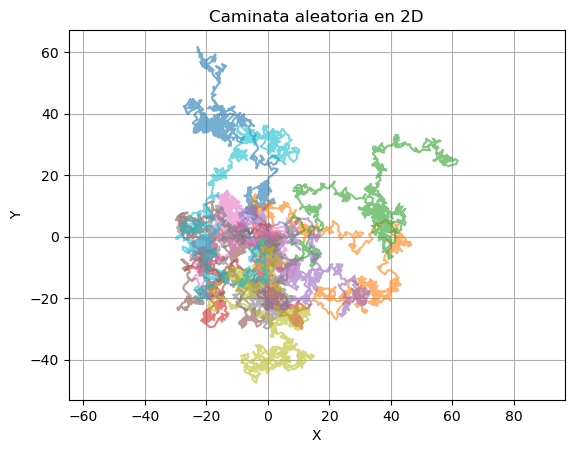
\includegraphics[width=0.9\linewidth]{imagenes/randomwalk.png}
    \caption{Generamos 10 caminatas aleatorias de 1000 pasos utilizando como semilla el generador lineal de congruencias.}
    \label{randomwalk}
\end{figure}

 Podemos calcular la distancia promedio al origen en función de $N$-ésimo paso dado, y ver el valor $R_N$ evoluciona (ver Fig. \ref{rvn}). Al calcular el valor de expectación y compararlo con el valor teórico esperado, debido a la naturaleza de la distribución elegida, vemos que $R_N \propto \sqrt{N}$ (ver Fig. \ref{rvsqrtn}).

\begin{figure}[!h]
    \centering
    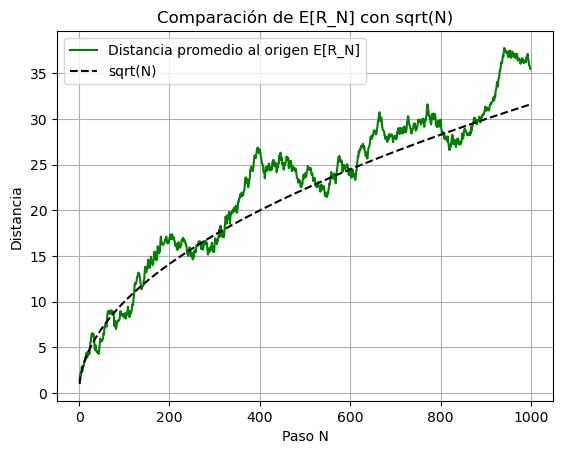
\includegraphics[width=0.9\linewidth]{imagenes/rvn.png}
    \caption{Distancia promedio al origen en función del paso $N$}
    \label{rvn}
\end{figure}

\begin{figure}[!h]
    \centering
    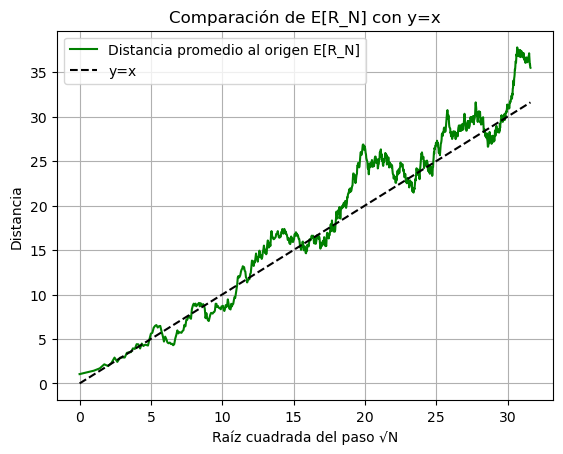
\includegraphics[width=0.9\linewidth]{imagenes/rvsqrtn.png}
    \caption{Distancia promedio al origen en función de $\sqrt{N}$}
    \label{rvsqrtn}
\end{figure}

\subsection{Generador de Fibonacci con Retardo}

Para poder funcionar, el generador de Fibonacci necesita una semilla, una implementación interesante seria usar de semilla nuestro generador lineal de congruencias para tener aun mas "aleatoriedad". Para esto se utiliza la función \texttt{rfx.fiboz()}, que genera $n$ números enteros aleatorios (ver Fig. \ref{fibo}), y \texttt{rfx.fibor()}, que genera $n$ números entre 0 y 1 (ver Fig. \ref{fibo01}). Ambas utilizando la función \texttt{rfx.gclr()} como base. 

\begin{figure}[!h]
    \centering
    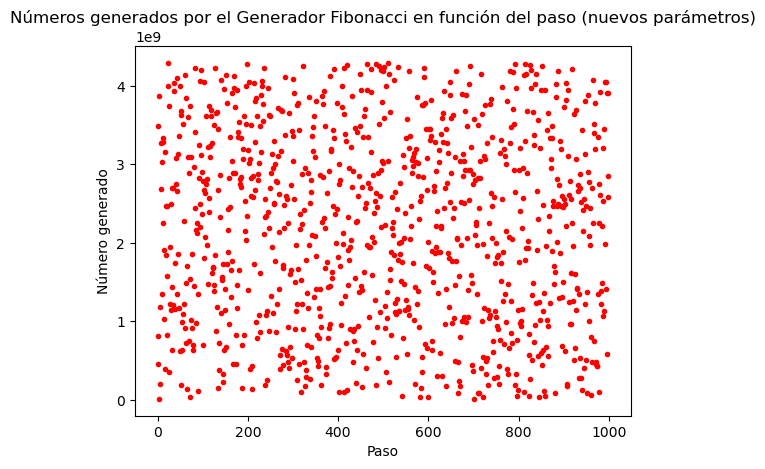
\includegraphics[width=0.9\linewidth]{imagenes/fibo.png}
    \caption{1000 números enteros, generados con la función \texttt{rfx.fiboz()}.}
    \label{fibo}
\end{figure}

\begin{figure}[!h]
    \centering
    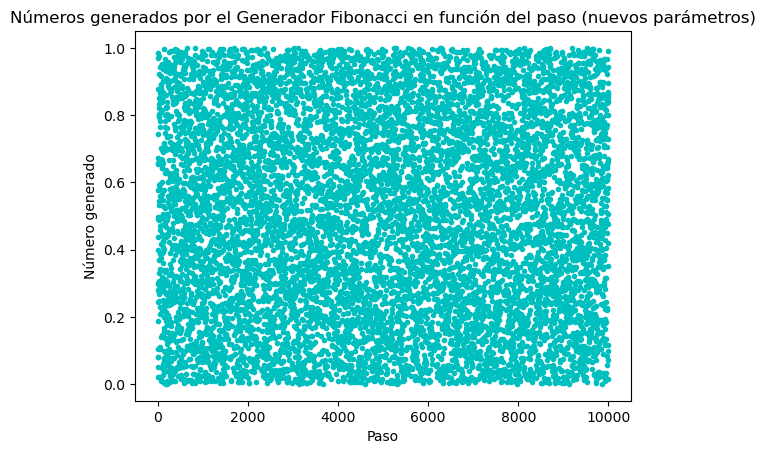
\includegraphics[width=0.9\linewidth]{imagenes/fibo01.png}
    \caption{5000 números entre 0 y 1, generados con la función \texttt{rfx.fibor()}.}
    \label{fibo01}
\end{figure}

Ahora quisieramos calcular la media y la varianza muestral para comparar con los valores teóricos esperados.

¿Cuales son los valores esperados?

Dada la Media sabemos que $\bar{X} = \frac{1}{n} \sum_{i=1}^{n} X_i$, y que $S^2 = \frac{1}{n-1} \sum_{i=1}^{n} (X_i - \bar{X})^2$, son los valores a calcular y comparar.

Utilizando funciones varias se termina por comparar ambos casos. Notamos que los errores relativos entre Media y Varianza son bastante pequeños, indicandonos que tenemos un buen generador (ver Tabla \ref{comparacion_fibo}).


\begin{table}[h!]
\centering
\footnotesize
\caption{Evaluación del generador de Fibonacci con retardo: comparación muestral vs teórico}
\label{comparacion_fibo}
\begin{tabular}{l S[table-format=1.6] S[table-format=1.6] S[table-format=1.2]@{\,}\%}
\toprule
& \textbf{Muestral} & \textbf{Teórico} & \textbf{Error} \\
\midrule
Media ($\mu$) & 0.499854 & 0.500000 & 0.03 \\
Varianza ($\sigma^2$) & 0.083345 & 0.083333 & 0.01 \\
\bottomrule
\end{tabular}
\end{table}

Ahora además queremos ver gráficamente como es el comportamiento, por lo propio buscamos visualizar un histograma que nos de cuenta de qué tan bueno es esto.

Notaremos una buena uniformidad nacida del hecho de que este es un buen generador de número aleatorio (ver Fig. \ref{fibohisto}).

\begin{figure}[!h]
    \centering
    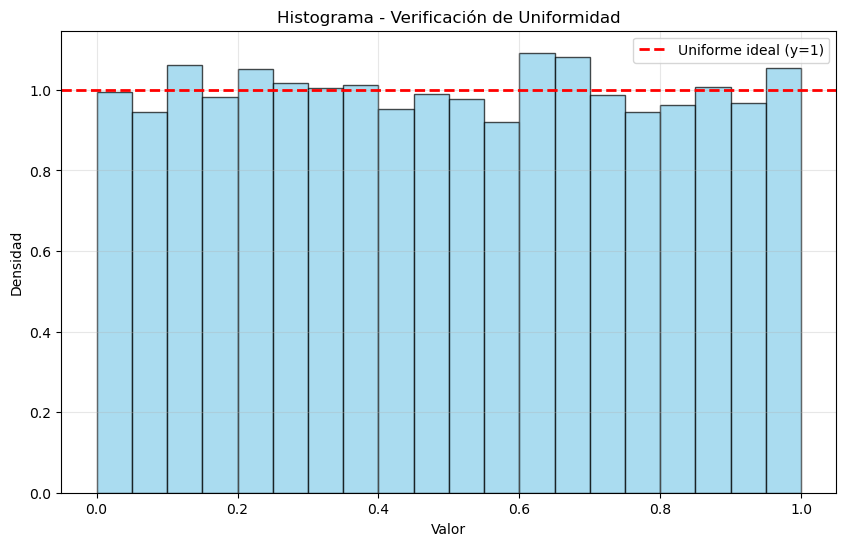
\includegraphics[width=0.9\linewidth]{imagenes/fibohisto.png}
    \caption{Histograma de la distribución generada por la función \texttt{rfx.fibor()}.}
    \label{fibohisto}
\end{figure}

La librería Numpy realiza esta tarea de forma automática mediante la función $\texttt{np.random.random()}$, ahora quisiéramos comparar ambos generadores para ver si son comparables o no, cuál es mejor, etc.

Podríamos decir sin ningún problema que ambos generan distribuciones uniformes (ver Fig. \ref{fibohistovnp}). salvo pequeñas variaciones/fluctuaciones alrededor del valor esperado. Recordemos que la convergencia se da a altísimos órdenes de magnitud. Con más números, las distribuciones serían prácticamente iguales.

\begin{figure}[!h]
    \centering
    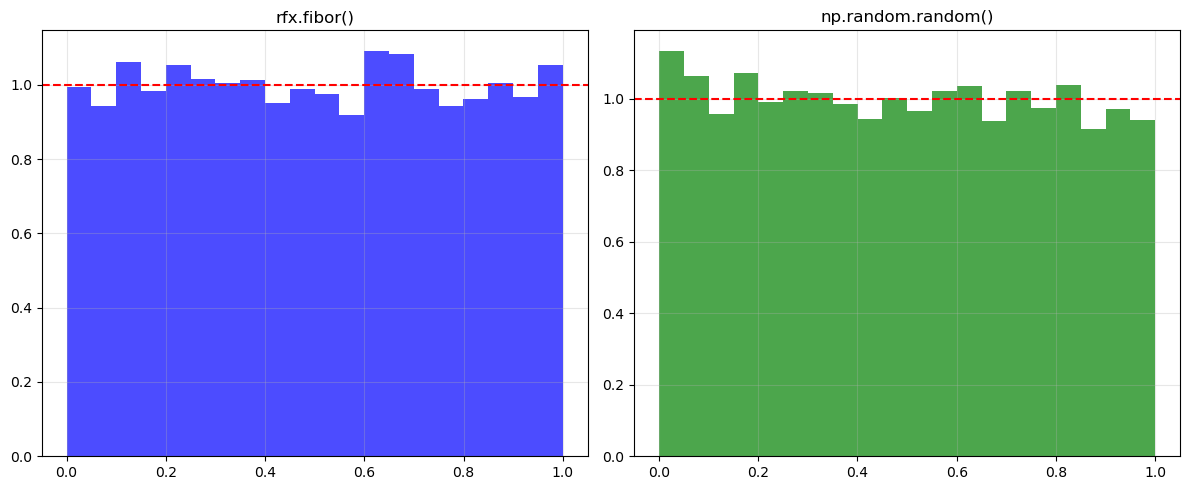
\includegraphics[width=0.9\linewidth]{imagenes/fibohistovnp.png}
    \caption{Histograma de la distribución generada comparada con una distribución generada por la función \texttt{np.random.random()}.}
    \label{fibohistovnp}
\end{figure}

\subsection{Coeficiente de Pearson para comparar correlaciones}

Generamos una función llamada \texttt{rfx.pearson()} que toma dos valores, $x$ e $y$ (en nuestro caso los generadores \texttt{rfx.gclr()} y \texttt{rfx.fibor()}), con la misma semilla y misma cantidad de numeros generados. Esta nos devuelve el valor de $r$, que en nuestro caso termina siendo: $r=0.013840$.

0.01384 está extremadamente cerca de 0. Esto quiere decir que no hay una asociación directa y no hay forma facil de predecir una variable basandote en la otra, ambas varian de forma independiente. Resultado curioso dado que $\texttt{rfx.fibor()}$ depende de una semilla generado por $\texttt{rfx.gclr()}$. Por lo tanto podemos intuir que ambos son buenos generadores.

\section{Resultados de Aplicaciones concretas}

A continuación utilizaremos las funciones creadas hasta ahora para modelar ciertas situaciones que necesiten de la aleatoriedad para funcionar.

\subsection{Problema de Monty Hall: Análisis por Simulación}

El problema de Monty Hall modela una situación donde un participante elige entre tres puertas, tras una de las cuales se oculta un premio. Tras la elección inicial, el presentador (que conoce la ubicación del premio) abre una puerta revelando un contenido no premiado, y ofrece cambiar de elección.

Definiendo los eventos:
\begin{itemize}
    \item $A$: Elección inicial correcta ($P(A) = 1/3$)
    \item $A^c$: Elección inicial incorrecta ($P(A^c) = 2/3$)
\end{itemize}
Las probabilidades condicionales son:
\[
P(\text{Ganar}|\text{No cambiar}) = P(A) = \frac{1}{3}
\]
\[
P(\text{Ganar}|\text{Cambiar}) = P(A^c) = \frac{2}{3}
\]
Se simuló el proceso $N=10^5$ veces usando generadores pseudoaleatorios:
\begin{itemize}
    \item Ubicación aleatoria del premio y elección inicial
    \item Presentador abre puerta con cabra
    \item Evaluación de ambas estrategias
\end{itemize}

La simulación valida el resultado teórico: cambiar de puerta aumenta la probabilidad de éxito del 33\% al 67\% (ver Tabla \ref{monty}).

\begin{table}[h]
    \centering
    \small
    \caption{Comparación de valores Teóricos vs. Simulados}
    \begin{tabular}{lcc}
        \toprule
        Estrategia & Prob. Teórica & Prob. Simulada \\
        \midrule
        No cambiar & 0.3333 & 0.3312 \\
        Cambiar & 0.6667 & 0.6688 \\
        \bottomrule
    \end{tabular}
    \label{monty}
    \vspace{0.5em}
\end{table}

\subsection{Generador de catálogos sintéticos de galaxias}

Supongamos que se quiere generar un catálogo sintético de galaxias donde los tipos morfológicos siguen una distribución de probabilidad específica: Elípticas (40\%), Espirales (30\%), Enanas (20\%) e Irregulares (10\%). Este modelo simula distribuciones reales observadas en surveys astronómicos.

La variable aleatoria $X$ representa el tipo de galaxia con distribución:
\begin{align*}
P(X = \text{Elíptica}) &= 0.4 \\
P(X = \text{Espiral}) &= 0.3 \\
P(X = \text{Enana}) &= 0.2 \\
P(X = \text{Irregular}) &= 0.1
\end{align*}
Se utiliza el método de transformada inversa para muestrear esta distribución discreta. Utilizamos para esto, dentro del propio notebook, las funciones generadoras de números aleatorios.

Para cada galaxia en el catálogo:
\begin{enumerate}
    \item Se genera $u$ entre 0 y 1
    \item Se asigna el tipo según:
    \[
    \text{Tipo} = 
    \begin{cases}
    \text{Elíptica} & u \in [0, 0.4) \\
    \text{Espiral} & u \in [0.4, 0.7) \\
    \text{Enana} & u \in [0.7, 0.9) \\
    \text{Irregular} & u \in [0.9, 1.0)
    \end{cases}
    \]
\end{enumerate}
Se generaron $N = 10^5$ galaxias usando un generador congruencial lineal. Los resultados obtenidos se condicen con las probabilidades esperadas (ver Tabla \ref{galax} y Fig \ref{galaxias}).

\begin{table}[h]
    \centering
    \small
    \caption{Probabilidad Teórica de encontrar una galaxia de cierto tipo vs. probabilidad simulada}
    \begin{tabular}{lccc}
        \toprule
        Tipo & Prob. Teórica & Prob. Simulada \\
        \midrule
        Elíptica & 0.4000 & 0.3949  \\
        Espiral & 0.3000 & 0.3037 \\
        Enana & 0.2000 & 0.2031 \\
        Irregular & 0.1000 & 0.0983 \\
        \bottomrule
    \end{tabular}
    \label{galax}
    \vspace{0.5em}
\end{table}

\begin{figure}[!h]
    \centering
    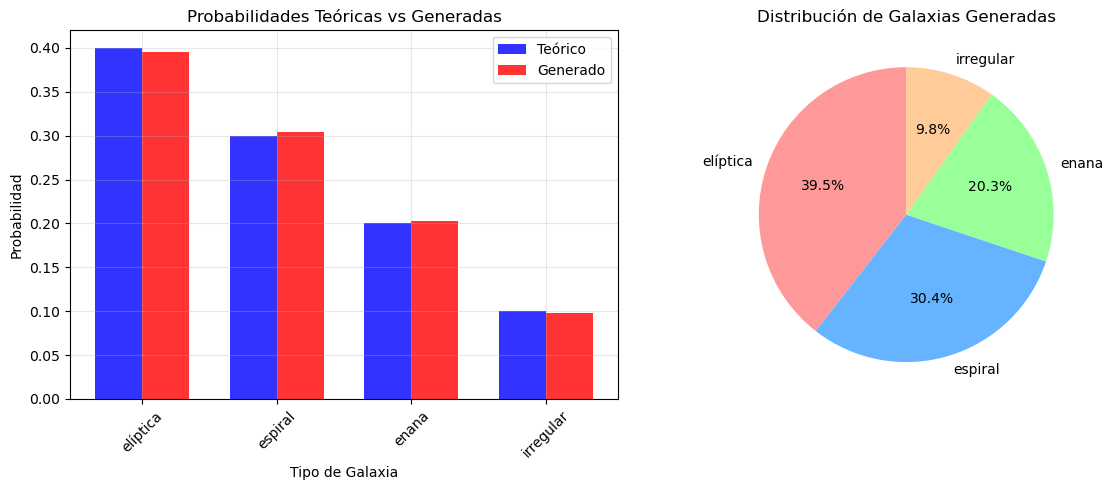
\includegraphics[width=1\linewidth]{imagenes/galaxias.png}
    \caption{Comparación de valores teóricos versus valores simulados para nuestro catálogo sintético de galaxias.}
    \label{galaxias}
\end{figure}

\subsection{Tirar dos dados: Expectativa vs. Realidad}

En este experimento se compara dos métodos de simulación para la variable aleatoria suma de dos dados equilibrados: (c) muestreo directo de la distribución teórica y (d) simulación empírica mediante lanzamientos individuales. Se evaluó la precisión de ambos métodos frente al modelo teórico.

Para dos dados equilibrados de seis caras, la suma \(S\) sigue una distribución discreta con:
\[
P(S = k) = \frac{6 - |k - 7|}{36}, \quad \text{para } k = 2, 3, \dots, 12
\]
Valores esperados: \(\mu = 7\), \(\sigma^2 = 5.833\).

\begin{itemize}
    \item \textbf{Método (c):} Muestreo directo de la distribución teórica usando transformada inversa
    \item \textbf{Método (d):} Simulación de lanzamientos individuales de dados (\(2 \times 10^4\) lanzamientos)
    \item Tamaño de muestra: \(N = 10,000\) realizaciones
    \item Generador utilizado: Congruencial lineal con parámetros optimizados
\end{itemize}

Obteniendo asi los resultados 

\begin{table}[!h]
    \centering
    \small
    \begin{tabular}{lcc}
        \toprule
        Métrica & Método (c) & Método (d) \\
        \midrule
         (MSE) & 0.000003 & 0.000010 \\
        Máx. dif. absoluta & 0.0046 & 0.0060 \\
        Media muestral & 6.997 & 7.003 \\
        Varianza muestral & 5.827 & 5.841 \\
        \bottomrule
    \end{tabular}
    \caption{Medida de errores y estadísticos}
    \label{dados_stat}
\end{table}


\begin{table*}[!h]
    \centering
    \footnotesize
    \begin{tabular}{lcccccc}
        \toprule
        Suma & Prob. Teórica & \multicolumn{2}{c}{Prob. Simulada} & \multicolumn{2}{c}{Diferencia} \\
        \cmidrule(lr){3-4} \cmidrule(lr){5-6}
        & & (c) Inversa & (d) Empírica & (c) & (d) \\
        \midrule
        2 & 0.0278 & 0.0279 & 0.0253 & 0.0001 & 0.0025 \\
        3 & 0.0556 & 0.0571 & 0.0517 & 0.0015 & 0.0039 \\
        4 & 0.0833 & 0.0837 & 0.0868 & 0.0004 & 0.0035 \\
        5 & 0.1111 & 0.1144 & 0.1118 & 0.0033 & 0.0007 \\
        6 & 0.1389 & 0.1388 & 0.1413 & 0.0001 & 0.0024 \\
        7 & 0.1667 & 0.1669 & 0.1727 & 0.0002 & 0.0060 \\
        8 & 0.1389 & 0.1387 & 0.1352 & 0.0002 & 0.0037 \\
        9 & 0.1111 & 0.1111 & 0.1069 & 0.0000 & 0.0042 \\
        10 & 0.0833 & 0.0833 & 0.0854 & 0.0000 & 0.0021 \\
        11 & 0.0556 & 0.0510 & 0.0560 & 0.0046 & 0.0004 \\
        12 & 0.0278 & 0.0271 & 0.0269 & 0.0007 & 0.0009 \\
        \bottomrule
    \end{tabular}
    \caption{Comparación de probabilidades teóricas y simuladas}
    \label{dados_resul}
\end{table*}


Ambos métodos reproducen adecuadamente la distribución teórica (ver Tabla \ref{dados_resul} y Fig. \ref{dados}), con el método (c) mostrando menor error cuadrático medio (MSE = 3e-6 vs 1e-5). La máxima diferencia absoluta fue de 0.0046 para el método (c) y 0.0060 para el (d). Los valores de media y varianza muestral coinciden con los teóricos (\(\mu = 7\), \(\sigma^2 = 5.833\)) dentro del margen esperado para \(N = 10,000\) (ver Tabla \ref{dados_stat}).

\begin{figure}[!h]
    \centering
    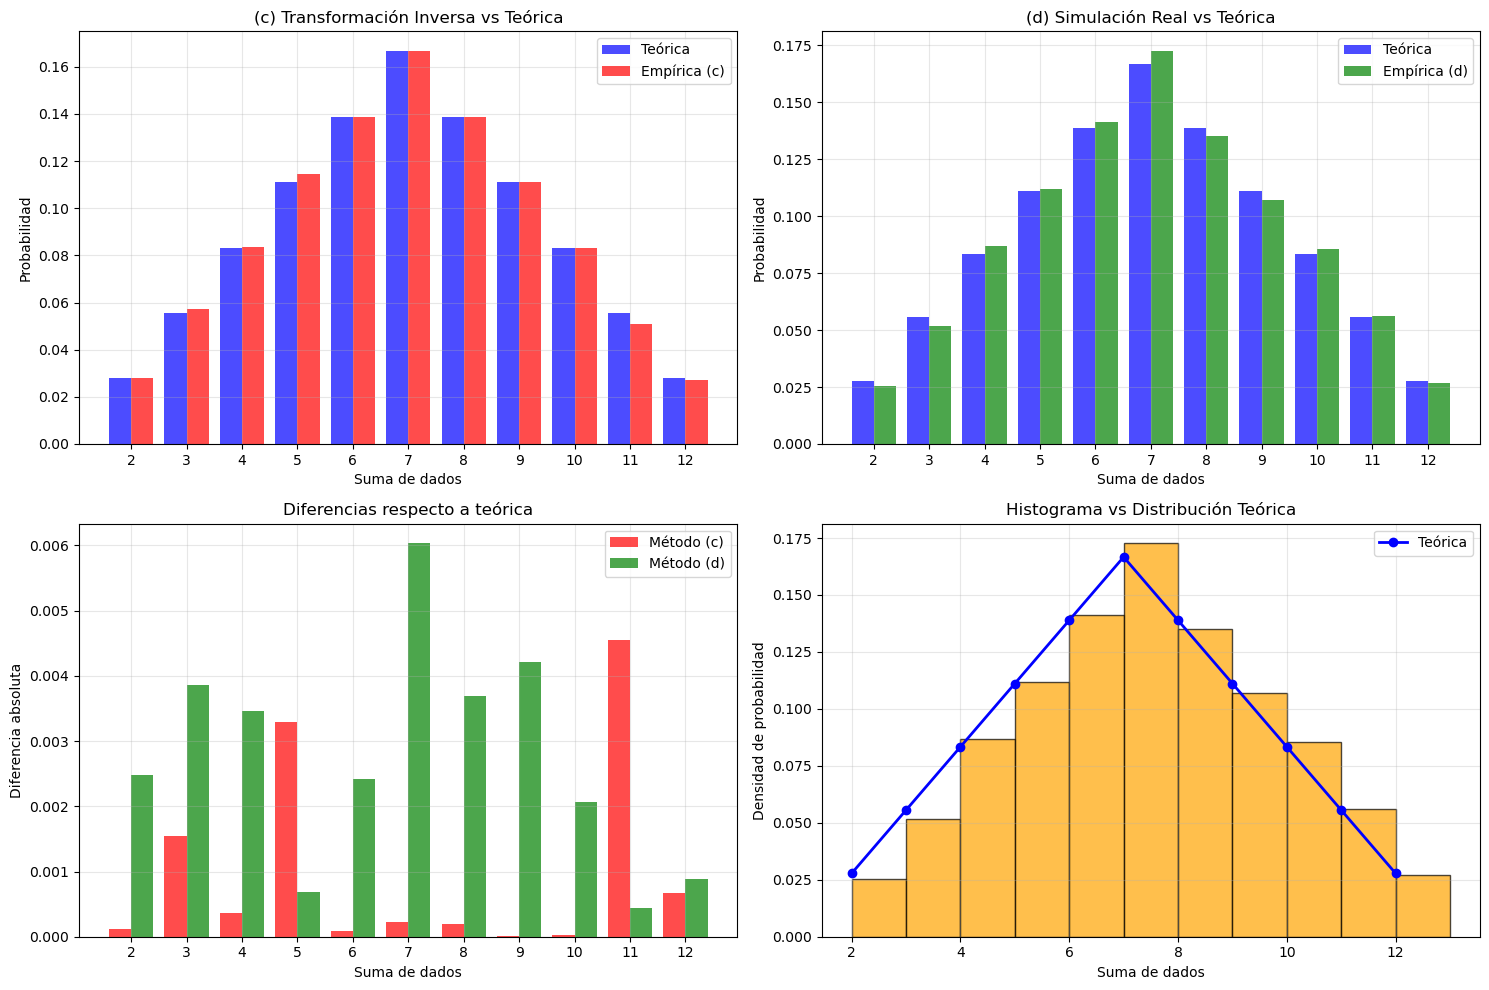
\includegraphics[width=1\linewidth]{imagenes/dados.png}
    \caption{Comparación entre metodos para calculo de valores medios y desviaciones esperadas.}
    \label{dados}
\end{figure}


\section{Conclusiones}
Se pudieron estudiar los comportamientos teóricos y empíricos de los generadores de números pseudoaleatorios propuestos. Se detecta que la uniformidad de los mismos es proporcional a la cantidad de muestras generadas.

Se lograron estudiar los momentos, cantidades asociadas a cada una de las distribuciones generadas, para posteriormente compararlas con los valores teóricos esperados. Pudimos asociar cada uno de estos a cantidades representativas de las distribuciones.

Estudiamos el Coeficiente de Pearson y lo calculamos para los dos generadores de números pseudoaleatorios creados. Concluimos que, pese a su relación, pues uno depende del otro para funcionar, su correlación es baja.

Se pudo implementar los generadores en diversos problemas, modelando situaciones reales como el juego de \textit{Monty Hall}, \textit{Tipos de galaxias} y \textit{Suma de dados}, para comparar estos con sus valores teóricos esperados. Para cada uno pudimos replicar de buena manera los valores teóricos esperados con valores simulados a través de algun algoritmo.

Para nuestro catálogo sintético el método de transformada inversa genera catálogos sintéticos que reproducen fielmente la distribución teórica. La técnica es aplicable a la creación de muestras artificiales para calibrar algoritmos de clasificación morfológica en astronomía.

En el caso de los dados el muestreo directo por transformada inversa (método c) demostró mayor precisión que la simulación empírica (método d), aunque ambos métodos son válidos para aplicaciones prácticas. Los resultados validan la efectividad de los generadores pseudoaleatorios para simular distribuciones de probabilidad discretas en contextos astronómicos y estadísticos.

Este trabajo logró cumplir satisfactoriamente los objetivos planteados, demostrando la efectividad de los métodos de simulación computacional para el estudio de sistemas estocásticos. A través de la implementación de generadores pseudoaleatorios (congruencial lineal y Fibonacci con retardo), se validaron conceptos probabilísticos fundamentales y se reprodujeron distribuciones teóricas con alta precisión.

Los resultados obtenidos en los diferentes ejercicios muestran consistencia entre las predicciones teóricas y las simulaciones empíricas, con errores cuadráticos medios del orden de $10^{-5}$ a $10^{-6}$. 


%%%%%%%%%%%%%%%%%%%%%%%%%%%%%%%%%%%%%%%%%%%%%%%%%%%%%%%%%%%%%%%%%%%%%%%%%%%%%%
%  ******************* Bibliografía / Bibliography ************************  %
%                                                                            %
%  -Ver en la sección 3 "Bibliografía" para mas información.                 %
%  -Debe usarse BIBTEX.                                                      %
%  -NO MODIFIQUE las líneas de la bibliografía, salvo el nombre del archivo  %
%   BIBTEX con la lista de citas (sin la extensión .BIB).                    %
%                                                                            %
%  -BIBTEX must be used.                                                     %
%  -Please DO NOT modify the following lines, except the name of the BIBTEX  %
%  file (without the .BIB extension).                                       %
%%%%%%%%%%%%%%%%%%%%%%%%%%%%%%%%%%%%%%%%%%%%%%%%%%%%%%%%%%%%%%%%%%%%%%%%%%%%%% 

\bibliographystyle{baaa}
\small
\bibliography{bibliografia}
%%%%%%%%%%%%%%%%%%%%%%%%%%%%%%%%%%%%%%%%%%%%%%%%%%%%%%%%%%%%%%%%%%%%%%%%%%%%%%%%%%%%%%%%%%%%%

%%%%%%%%%%%%%%%%%%%%%%%%APENDICES%%%%%%%%%%%%%%%%%%%%%%%%


\end{document}
